\documentclass{uebblatt}
\usepackage{wrapfig}

\newcommand{\http}{http:/\kern-.2em/\kern-0.03em}

\begin{document}

\maketitle{0}{\emph{Präsenzblatt für die erste Übung}}

\begin{aufgabe*}{Geometrische Reihe in der Algebra}
\begin{enumerate}
\item Sei~$x$ ein nilpotentes Element eines kommutativen Rings~$A$. Zeige,
dass~$1-x$ eine Einheit ist.
\item Folgere: Die Summe eines nilpotenten Elements mit einer Einheit ist
wieder eine Einheit.
\end{enumerate}
\end{aufgabe*}

\begin{aufgabe*}{Idealkarten wichtiger Ringe}
Zeichne für die folgenden Ringe eine Übersicht über ihre Ideale. Welche sind
maximal, welche prim?
\begin{enumerate}
\item $\ZZ$
\item $k$ (dabei ist~$k$ ein beliebiger Körper)
\item $\CC[X]$
\item $\RR[X]$
\end{enumerate}
\end{aufgabe*}

\begin{aufgabe*}{Minimale Primideale}
Sei~$\ppp$ ein Primideal in einem kommutativen Ring. Zeige, dass es unter den
Primidealen~$\qqq$ mit~$\qqq \subseteq \ppp$ ein minimales gibt.
\end{aufgabe*}

\vfill
\begin{center}
  \rotatebox{90}{\tiny\sffamily \http spikedmath.com/392.html}
  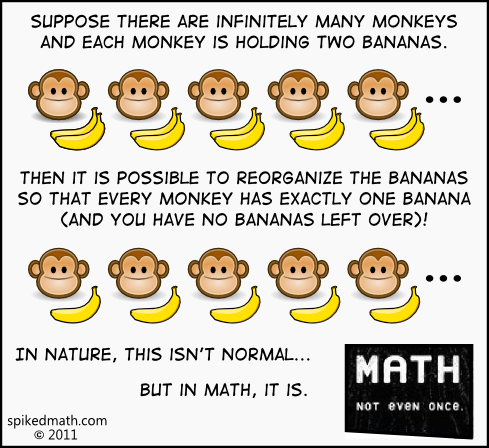
\includegraphics[height=3.7cm]{images/math-not-even-once}
  \qquad
  \rotatebox{90}{\tiny\sffamily \http xkcd.com/982/}
  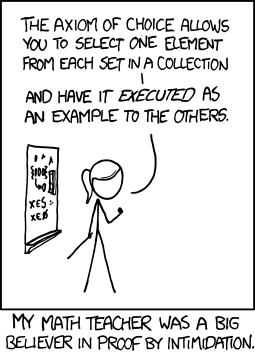
\includegraphics[height=3.7cm]{images/axiom-of-choice}
  \qquad
  \rotatebox{90}{\tiny\sffamily \http spikedmath.com/198.html}
  
\includegraphics[height=3.7cm]{images/please-think-of-the-kittens}
\end{center}

\end{document}
